\section{Existerande Raviolimaskiner}
De Raviolimaskiner som finns på marknad innehåller två huvuddelar, en pump för fyllning och en motor-driven degform. 

Ett exempel på en Raviolimaskin visas på Figuren~\ref{raviolihemma}. Den består av två cylindriska degformar och en lucka där man fyller maskinen med fyllningsmaterial. Maskinens degfomar fungerar även som pump genom att de drar in fyllningsmaterialet när man snurrar dem m.h.a. ett handtag eller en motor.
 	\begin{figure}[h]
 		\begin{center}
 			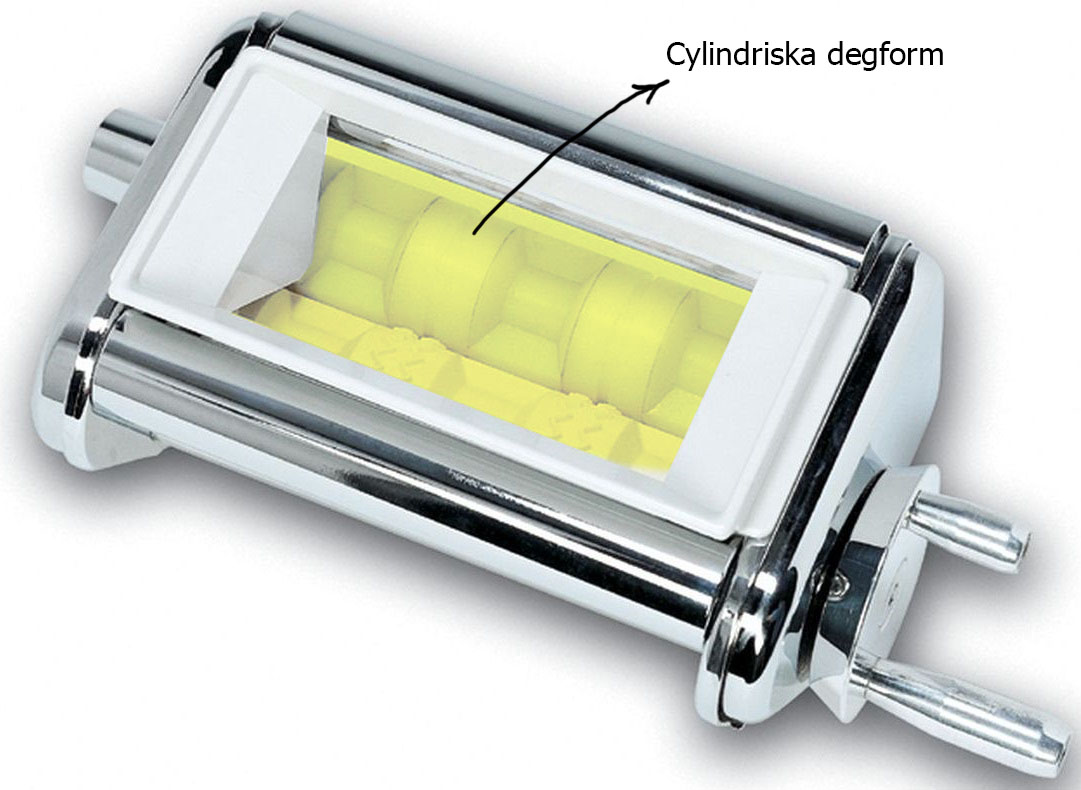
\includegraphics[scale=0.4]{images/ravioli_machine_comment.jpg}
 			\caption{Raviolimaskin bestående av två cylindriska degformar }
 			\label{raviolihemma}	
 		\end{center}
 	\end{figure}
 
Ett annat exempel på en industriell Raviolimaskin visas på figur ~\ref{industraviol_2}. Denna maskin består av en pump, två cylindriska degformar och en rullbana. Maskinen fungerar med samma princip som maskinen på det första exemplet gör och den fyller Raviolin oavbrutet under tiden som  Raviolidegen eller fyllningsmaterialet i pumpen inte har tagit slut.   .
 \begin{figure}[ht]
 	\begin{center}
 		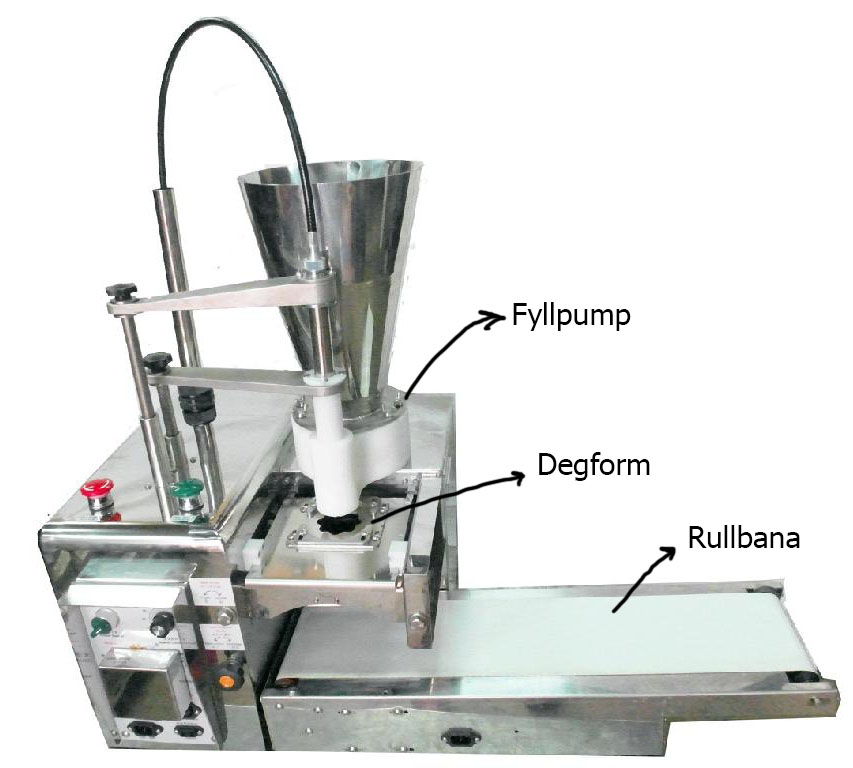
\includegraphics[scale=0.4]{images/industriell_machine_comment.jpg}
 		\caption{Industriell Raviolimaskin som gör en Ravioli i tag(ref)}
 		\label{industraviol_2}	
 	\end{center}
 \end{figure}
 
 

 